\documentclass[aspectratio=169,10pt]{beamer}
\usepackage{fontspec}
\setmainfont{Arial}
\IfFontExistsTF{Noto Sans CJK SC}{\newfontfamily\cjkfont{Noto Sans CJK SC}}{\newfontfamily\cjkfont[Path=/System/Library/Fonts/]{STHeiti Medium.ttc}}
\newcommand{\zh}[1]{{\cjkfont #1}}
\usepackage{amsmath,amssymb,booktabs,mathtools}
\usepackage{tikz}
\usetikzlibrary{arrows.meta,positioning,calc,fit,shapes.geometric}
\usepackage{graphicx}
\usepackage{hyperref}

\definecolor{navy}{HTML}{0B172A}
\definecolor{navy2}{HTML}{12243D}
\definecolor{ink}{HTML}{E6EEF7}
\definecolor{muted}{HTML}{A9B8C9}
\definecolor{teal}{HTML}{2DD4BF}
\definecolor{orange}{HTML}{F59E0B}
\definecolor{blue}{HTML}{60A5FA}
\definecolor{rose}{HTML}{FB7185}
\definecolor{green}{HTML}{86EFAC}
\definecolor{line}{HTML}{33465E}

\setbeamercolor{background canvas}{bg=navy}
\setbeamercolor{normal text}{fg=ink,bg=navy}
\setbeamercolor{frametitle}{fg=ink,bg=navy}
\setbeamercolor{title}{fg=ink}
\setbeamercolor{subtitle}{fg=muted}
\setbeamercolor{author}{fg=muted}
\setbeamercolor{date}{fg=muted}
\setbeamertemplate{navigation symbols}{}
\setbeamertemplate{frametitle}{\vspace{0.35cm}\insertframetitle\par\vspace{0.08cm}\color{teal}\rule{1.25cm}{1.2pt}\vspace{0.15cm}}
\setbeamertemplate{footline}{\hfill\color{muted}\scriptsize\insertframenumber\hspace{0.35cm}\vspace{0.2cm}}
\setbeamerfont{frametitle}{size=\Large,series=\bfseries}
\setbeamerfont{title}{size=\Huge,series=\bfseries}
\setbeamerfont{subtitle}{size=\large}
\setbeamerfont{normal text}{size=\small}
\setbeamertemplate{itemize item}{\color{teal}$\blacktriangleright$}
\setbeamertemplate{itemize subitem}{\color{orange}$\bullet$}
\newcommand{\source}[1]{\vspace{0.1cm}{\tiny\color{muted}Source: #1}}
\newcommand{\tagline}[1]{\textcolor{teal}{\textbf{#1}}}
\newcommand{\metric}[2]{\textcolor{#1}{\Large\bfseries #2}}

\begin{document}

% 1
\begin{frame}[plain]
  \vfill
  {\color{teal}\small EXPERIMENTAL RESEARCH PREVIEW \hspace{0.2cm} | \hspace{0.2cm} TASK 1--6}
  \vspace{0.28cm}
  {\usebeamerfont{title}\color{ink}Diagram Compiler\par}
  \vspace{0.15cm}
  {\usebeamerfont{subtitle}\color{muted}From fixed-order physics graphs to validated native kernels\par}
  \vspace{0.28cm}
  {\large\color{ink}\zh{物理感知图编译器：从图表示到可验证原生内核}\par}
  \vfill
  \resizebox{\linewidth}{!}{%

\begin{tikzpicture}
    \draw[teal,line width=2pt] (0,0) -- (2.3,0);
    \draw[orange,line width=2pt] (2.55,0) -- (4.5,0);
    \node[anchor=west, text=muted, font=\small] at (4.8,0) {LEVEL 2 validation | P1 unchanged | no speedup claim};
  \end{tikzpicture}%
}
  \vspace{0.3cm}
  {\tiny\color{muted}Darren Wong Ka Wa \quad 20 September 2026}
\end{frame}

% 2
\begin{frame}[shrink=8]{Theory background: the expensive object is a structured graph sum}
\begin{columns}[T,totalwidth=\textwidth]
\column{0.55\textwidth}
\vspace{0.2cm}
\begingroup\small
\begin{align*}
 F_n(x) &= \left(\frac{g}{\sqrt L}\right)^{2n}
 \sum_{C\in\mathcal C_n}
 \prod_{\text{electron segments}} G\;
 \prod_{\text{phonon chords}} D \\
 G(p,\Delta\tau)&=e^{-\xi_p\Delta\tau},\qquad
 D(\Delta\tau)=e^{-\omega\Delta\tau},\\[-0.1cm]
 \xi_k&=2t(1-\cos k)
\end{align*}
\endgroup
\vspace{0.15cm}
\resizebox{\linewidth}{!}{%

\begin{tikzpicture}[node distance=0.65cm]
  \node[draw=teal!70,fill=navy2,rounded corners=2pt,minimum width=2.5cm,minimum height=0.65cm] (h) {Hamiltonian};
  \node[draw=blue!70,fill=navy2,rounded corners=2pt,minimum width=2.5cm,minimum height=0.65cm,right=of h] (d) {Diagrams};
  \node[draw=orange!80,fill=navy2,rounded corners=2pt,minimum width=2.5cm,minimum height=0.65cm,right=of d] (o) {Observable};
  \draw[-{Latex[length=2mm]},thick,muted] (h)--(d);
  \draw[-{Latex[length=2mm]},thick,muted] (d)--(o);
\end{tikzpicture}%
}
\column{0.42\textwidth}
\vspace{0.1cm}
\textcolor{orange}{\bfseries Why software structure matters}
\begin{itemize}
  \item Pairings grow factorially with order.
  \item Different diagrams reuse the same propagator, vertex and momentum subexpressions.
  \item Two-band graphs add noncommutative matrix products and traces.
  \item Delayed acceptance needs a cheap state weight, then an exact correction.
\end{itemize}
\vspace{0.15cm}
\textcolor{muted}{The method starts by making the physics object explicit.}
\end{columns}
\source{Task 1 report; signed dispersion convention is frozen in the Future B constraints.}
\end{frame}


\begin{frame}{Real-material software workflow}
\begin{center}
\resizebox{\linewidth}{!}{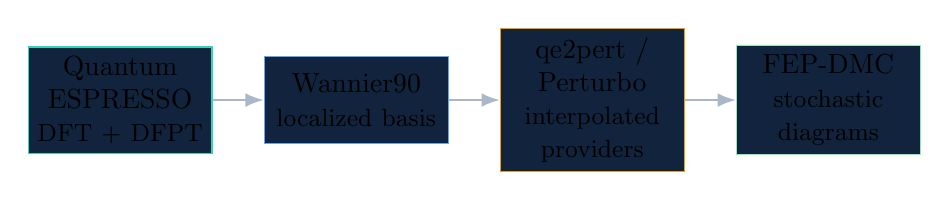
\begin{tikzpicture}[node distance=0.65cm]
\node[draw=teal,fill=navy2,text width=2.1cm,align=center,minimum height=1.1cm] (qe) {Quantum ESPRESSO\\\small DFT + DFPT};
\node[draw=blue,fill=navy2,text width=2.1cm,align=center,minimum height=1.1cm,right=of qe] (w) {Wannier90\\\small localized basis};
\node[draw=orange,fill=navy2,text width=2.1cm,align=center,minimum height=1.1cm,right=of w] (p) {qe2pert / Perturbo\\\small interpolated providers};
\node[draw=green,fill=navy2,text width=2.1cm,align=center,minimum height=1.1cm,right=of p] (d) {FEP-DMC\\\small stochastic diagrams};
\foreach \a/\b in {qe/w,w/p,p/d}{\draw[-{Latex},thick,muted](\a)--(\b);}
\end{tikzpicture}}
\end{center}
\vspace{0.25cm}
\[
H_{e\text{-}ph}=\sum_{nk}\epsilon_{nk}c^\dagger_{nk}c_{nk}
 +\sum_{\nu q}\hbar\omega_{\nu q}b^\dagger_{\nu q}b_{\nu q}
 +\frac{1}{\sqrt{N_q}}\sum_{mnkq\nu}g_{mn\nu}(k,q)c^\dagger_{m,k+q}c_{nk}
 (b_{\nu q}+b^\dagger_{\nu,-q}) .
\]
\small
Material calculations supply $\epsilon$, $\omega$ and $g$. The diagram sampler combines these factors with its measure and updates. Our present compiler supplies bounded analytic kernels, with a material-provider extension still required.
\source{\href{https://perturbo-code.github.io/mydoc_qe2pert.html}{Perturbo: QE to Perturbo}; \href{https://github.com/yaoluo/FEP-DMC}{FEP-DMC repository}. Workflow is schematic, not a completed compiler material run.}
\end{frame}

% 3
\begin{frame}[shrink=8]{Method object: one semantic IR, two execution paths}
\begin{center}
\resizebox{\linewidth}{!}{%
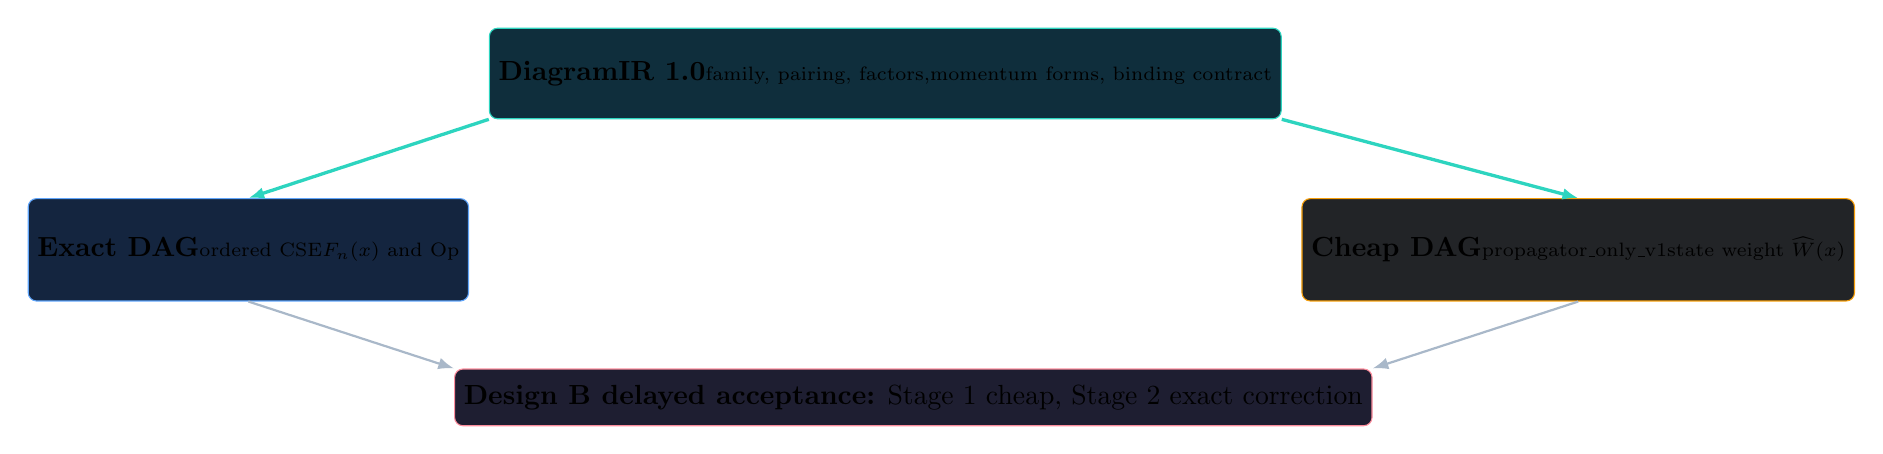
\begin{tikzpicture}[node distance=0.65cm and 0.7cm]
  \node[draw=teal,fill=teal!12!navy,rounded corners=3pt,minimum width=4.1cm,minimum height=1.15cm,align=center] (ir) {\textbf{DiagramIR 1.0}\par\scriptsize family, pairing, factors,\par momentum forms, binding contract};
  \node[draw=blue,fill=blue!10!navy,rounded corners=3pt,minimum width=3.2cm,minimum height=1.3cm,below left=1.0cm and 0.25cm of ir,align=center] (exact) {\textbf{Exact DAG}\par\scriptsize ordered CSE\par $F_n(x)$ and $\mathrm{Op}$};
  \node[draw=orange,fill=orange!10!navy,rounded corners=3pt,minimum width=3.2cm,minimum height=1.3cm,below right=1.0cm and 0.25cm of ir,align=center] (cheap) {\textbf{Cheap DAG}\par\scriptsize propagator\_only\_v1\par state weight $\widehat W(x)$};
  \draw[-{Latex[length=2mm]},very thick,teal] (ir.south west) -- (exact.north);
  \draw[-{Latex[length=2mm]},very thick,teal] (ir.south east) -- (cheap.north);
  \node[draw=rose!80,fill=rose!8!navy,rounded corners=3pt,minimum width=7.2cm,minimum height=0.72cm,below=0.85cm of $(exact.south)!0.5!(cheap.south)$,align=center] (da) {\textbf{Design B delayed acceptance:} Stage 1 cheap, Stage 2 exact correction};
  \draw[-{Latex[length=2mm]},thick,muted] (exact.south) -- (da.north west);
  \draw[-{Latex[length=2mm]},thick,muted] (cheap.south) -- (da.north east);
\end{tikzpicture}%
}
\end{center}
\vspace{0.3cm}
\begin{columns}[T,totalwidth=\textwidth]
\column{0.48\textwidth}
\tagline{What is new in the method}\par
The same physical representation feeds exact evaluation, cheap screening and native lowering. The approximation is declared by policy rather than hidden in duplicated code.
\column{0.48\textwidth}
\tagline{Scope}\par
Fixed-order scalar Holstein and Hermitian two-band families. The graph counts show structural reuse, not a generic compiler or an automatic speedup result.
\end{columns}
\source{Task 1--3 reports; Task 2 explicitly records no scalar wall-clock claim.}
\end{frame}

% 4
\begin{frame}{Compiler pipeline: from physics contract to native validation}
\begin{center}
\resizebox{\linewidth}{!}{%
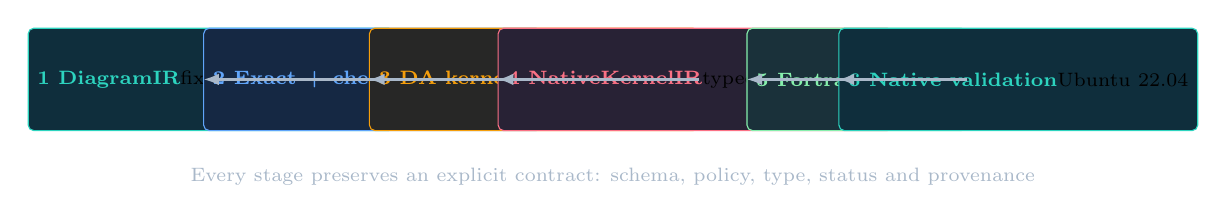
\begin{tikzpicture}[x=1cm,y=1cm]
\foreach \x/\c/\t/\s/\id in {
0/teal/1 DiagramIR/fixed-order semantics/1,
2.05/blue/2 Exact + cheap/ordered DAGs/2,
4.1/orange/3 DA kernel/Design B + target/3,
6.15/rose/4 NativeKernelIR/typed SSA + CFG/4,
8.2/green/5 Fortran/fortran\_v1/5,
10.25/teal/6 Native validation/Ubuntu 22.04/6}
{
  \node[draw=\c,fill=\c!12!navy,rounded corners=2pt,minimum width=1.72cm,minimum height=1.3cm,align=center,font=\scriptsize] (n\id) at (\x,0) {\textcolor{\c}{\bfseries \t}\par \s};
}
\foreach \a/\b in {n1/n2,n2/n3,n3/n4,n4/n5,n5/n6}{\draw[-{Latex[length=2mm]},very thick,muted] (\a.east)--(\b.west);}
\node[anchor=north,align=center,text=muted,font=\scriptsize] at (5.1,-1.0) {Every stage preserves an explicit contract: schema, policy, type, status and provenance};
\end{tikzpicture}%
}
\end{center}
\vspace{0.45cm}
\begin{columns}[T,totalwidth=\textwidth]
\column{0.48\textwidth}
\textcolor{teal}{\bfseries Software-package process}\par
Source modules \(\rightarrow\) JSON artifacts \(\rightarrow\) executable scripts \(\rightarrow\) differential tests \(\rightarrow\) Docker/CI \(\rightarrow\) prerelease evidence bundle.
\column{0.48\textwidth}
\textcolor{orange}{\bfseries Scientific boundary}\par
Task 6 uses a separate validation executable. It does not wire the generated kernel into production \texttt{update\_swap} or public P1.
\end{columns}
\source{Task 4--6 reports; Task 6 integration architecture A.}
\end{frame}

% 5
\begin{frame}{Structural reuse is visible before timing}
\begin{columns}[T,totalwidth=\textwidth]
\column{0.62\textwidth}
\resizebox{\linewidth}{!}{%
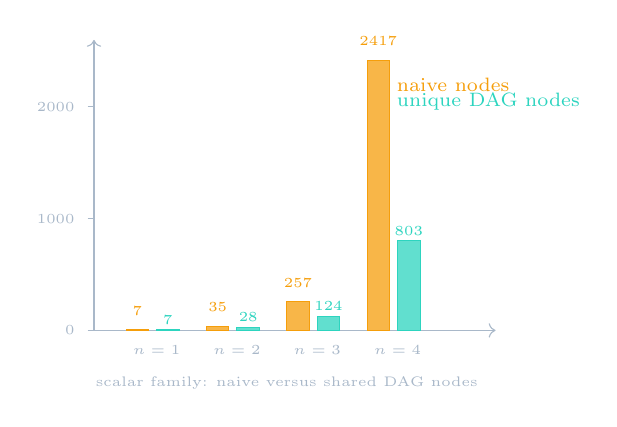
\begin{tikzpicture}[x=1.02cm,y=0.00142cm]
  \draw[->,muted] (-0.4,0)--(4.6,0);
  \draw[->,muted] (-0.4,0)--(-0.4,2600);
  \foreach \y/\lab in {0/0,1000/1000,2000/2000}{\draw[muted] (-0.48,\y)--(-0.4,\y);\node[anchor=east,font=\tiny,text=muted] at (-0.52,\y) {\lab};}
  \foreach \x/\n/\d/\lab in {0/7/7/1,1/35/28/2,2/257/124/3,3/2417/803/4}{
    \pgfmathsetmacro{\xx}{\x+0.38}
    \draw[fill=orange!75,draw=orange] (\x,0) rectangle ++(0.28,\n);
    \draw[fill=teal!75,draw=teal] (\xx,0) rectangle ++(0.28,\d);
    \node[font=\tiny,text=muted] at (\xx,-180) {$n=\lab$};
    \node[font=\tiny,text=orange] at (\x+0.14,\n+170) {\n};
    \node[font=\tiny,text=teal] at (\xx+0.14,\d+90) {\d};
  }
  \node[font=\scriptsize,text=orange,anchor=west] at (3.25,2200) {naive nodes};
  \node[font=\scriptsize,text=teal,anchor=west] at (3.25,2050) {unique DAG nodes};
  \node[font=\tiny,text=muted,anchor=north] at (2.0,-330) {scalar family: naive versus shared DAG nodes};
\end{tikzpicture}%
}
\column{0.35\textwidth}
\textcolor{teal}{\bfseries Two-band expensive primitives}\par
\vspace{0.12cm}
\begin{tabular}{c|rr}
\toprule
order $n$ & exact & cheap\\
\midrule
1 & 7 & 0\\
2 & 28 & 0\\
3 & 110 & 0\\
\bottomrule
\end{tabular}
\vspace{0.25cm}
\small
The cheap path removes matrix primitives by policy. This is a structural reduction. It is not reported as a speedup.
\end{columns}
\source{Task 1 graph\_stats.csv and Task 2 graph\_costs.csv.}
\end{frame}

% 6
\begin{frame}[shrink=8]{Exact-preserving delayed acceptance}
\begin{columns}[T,totalwidth=\textwidth]
\column{0.51\textwidth}
\begingroup\small
\begin{align*}
\widehat\ell &= \log\widehat W(y)-\log\widehat W(x),\\
\ell_R &= \log\pi(y)-\log\pi(x)+\log q(y,x)-\log q(x,y),\\
\alpha_1 &= \min\{1,e^{\widehat\ell}\},\\
\alpha_2 &= \min\{1,e^{\ell_R-\widehat\ell}\}.
\end{align*}
\endgroup
\vspace{0.12cm}
\resizebox{\linewidth}{!}{%
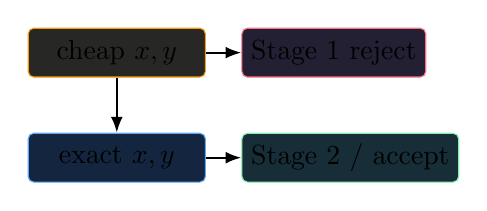
\begin{tikzpicture}[node distance=0.45cm]
  \node[draw=orange,fill=orange!12!navy,rounded corners=2pt,minimum width=2.25cm,minimum height=0.62cm,align=center] (c) {cheap $x,y$};
  \node[draw=rose,fill=rose!10!navy,rounded corners=2pt,minimum width=2.25cm,minimum height=0.62cm,align=center,right=of c] (r) {Stage 1 reject};
  \node[draw=blue,fill=blue!10!navy,rounded corners=2pt,minimum width=2.25cm,minimum height=0.62cm,align=center,below=0.7cm of c] (e) {exact $x,y$};
  \node[draw=green,fill=green!10!navy,rounded corners=2pt,minimum width=2.25cm,minimum height=0.62cm,align=center,right=of e] (a) {Stage 2 / accept};
  \draw[-{Latex[length=2mm]},thick] (c)--(r);
  \draw[-{Latex[length=2mm]},thick] (c)--(e);
  \draw[-{Latex[length=2mm]},thick] (e)--(a);
\end{tikzpicture}%
}
\column{0.42\textwidth}
\textcolor{orange}{\bfseries Target policy}\par
\texttt{positive\_real\_F\_v1}: \(\pi=F\) only when \(F\) is finite, real and positive. \(\lvert F\rvert\), complex modulus and \(F^2\) are refused.
\vspace{0.22cm}
\resizebox{\linewidth}{!}{\begin{tabular}{l|cc}
\toprule
proposal & balance & stationarity\\
\midrule
symmetric & $1.39\times10^{-17}$ & $0$\\
asymmetric & $1.39\times10^{-17}$ & $2.78\times10^{-17}$\\
\bottomrule
\end{tabular}}
\end{columns}
\vspace{0.15cm}
\tagline{Why it matters:} cheap rejection saves exact work while Stage 2 repairs the target and Hastings ratio.
\source{Task 3 finite-state balance evidence.}
\end{frame}

% 7
\begin{frame}{Native backend: typed lowering, deterministic Fortran, differential checks}
\begin{center}
\resizebox{\linewidth}{!}{%

\begin{tikzpicture}[node distance=0.52cm and 0.72cm]
\node[draw=teal,fill=teal!12!navy,rounded corners=2pt,minimum width=2.8cm,minimum height=0.9cm,align=center] (nir) {NativeKernelIR\par\scriptsize types + SSA + CFG};
\node[draw=orange,fill=orange!12!navy,rounded corners=2pt,minimum width=2.8cm,minimum height=0.9cm,align=center,right=of nir] (f) {Fortran\par\scriptsize fortran\_v1};
\node[draw=blue,fill=blue!12!navy,rounded corners=2pt,minimum width=2.8cm,minimum height=0.9cm,align=center,right=of f] (g) {gfortran 11.4\par\scriptsize Ubuntu 22.04};
\node[draw=green,fill=green!12!navy,rounded corners=2pt,minimum width=2.8cm,minimum height=0.9cm,align=center,right=of g] (v) {Oracle comparison\par\scriptsize 10 fixtures};
\foreach \a/\b in {nir/f,f/g,g/v}{\draw[-{Latex[length=2mm]},very thick,muted] (\a)--(\b);}
\end{tikzpicture}%
}
\end{center}
\vspace{0.35cm}
\begin{columns}[T,totalwidth=\textwidth]
\column{0.31\textwidth}\metric{teal}{224/224}\par exact cases\par\vspace{0.1cm}\metric{orange}{0}\par exact calls on Stage 1 reject
\column{0.31\textwidth}\metric{blue}{$6.66\times10^{-16}$}\par max primitive error\par\vspace{0.1cm}\metric{green}{0}\par native stationarity residual
\column{0.31\textwidth}\metric{rose}{ff4aa2de...}\par generated source SHA\par\vspace{0.1cm}\metric{teal}{LEVEL 2}\par FEP-DMC toolchain validation
\end{columns}
\vspace{0.3cm}
\small\color{muted}The native executable is a separate validation path. It does not replace production \texttt{update\_swap}.
\source{Task 5 primitive differential; Task 6 native differential and provenance.}
\end{frame}

% 8
\begin{frame}{Two software processes: conventional packaging and physics-aware packaging}
\begin{center}
\small\renewcommand{\arraystretch}{1.0}
\begin{tabular}{p{0.27\textwidth} p{0.31\textwidth} p{0.31\textwidth}}
\toprule
 & \textcolor{muted}{Conventional numerical package} & \textcolor{teal}{Our diagram compiler package}\\
\midrule
Core object & API calls and arrays & Explicit DiagramIR with physics contracts\\
Optimization & Local code paths & Ordered DAG sharing from the same IR\\
Approximation & Implementation detail & Versioned CheapPolicy and target policy\\
Correctness & Unit tests & Independent oracle and differential tests\\
Native path & Compile source & NativeKernelIR, ABI, status and laziness\\
Release evidence & Source plus tests & JSON provenance, Docker rebuild, pin, checksum bundle\\
\bottomrule
\end{tabular}
\end{center}
\source{Task 7 reproducibility repair and evidence bundle.}
\end{frame}

% 9
\begin{frame}{Connecting real materials: the next adapter boundary}
\begin{center}
\resizebox{\linewidth}{!}{%

\begin{tikzpicture}[node distance=0.58cm and 0.55cm]
\node[draw=teal,fill=teal!12!navy,rounded corners=2pt,minimum width=2.35cm,minimum height=1.0cm,align=center] (m) {material inputs\par\scriptsize bands, modes, couplings, gauge};
\node[draw=blue,fill=blue!12!navy,rounded corners=2pt,minimum width=2.35cm,minimum height=1.0cm,align=center,right=of m] (p) {provider adapter\par\scriptsize BindingLayout + units};
\node[draw=orange,fill=orange!12!navy,rounded corners=2pt,minimum width=2.35cm,minimum height=1.0cm,align=center,right=of p] (q) {physical graph\par\scriptsize propagator, vertex, measure};
\node[draw=rose,fill=rose!12!navy,rounded corners=2pt,minimum width=2.35cm,minimum height=1.0cm,align=center,right=of q] (v) {independent checks\par\scriptsize oracle + reverse move};
\node[draw=green,fill=green!12!navy,rounded corners=2pt,minimum width=2.35cm,minimum height=1.0cm,align=center,right=of v] (n) {native consumer\par\scriptsize shadow, then full observable};
\foreach \a/\b in {m/p,p/q,q/v,v/n}{\draw[-{Latex[length=2mm]},very thick,muted] (\a)--(\b);}
\end{tikzpicture}%
}
\end{center}
\vspace{0.32cm}
\begin{columns}[T,totalwidth=\textwidth]
\column{0.48\textwidth}
\textcolor{teal}{\bfseries Required gates}\par
\begin{itemize}
\item same Hamiltonian and units
\item measure, Jacobian and reverse proposal
\item target policy valid on the sampled domain
\item independent reference and native source pin
\end{itemize}
\column{0.48\textwidth}
\textcolor{orange}{\bfseries Current boundary}\par
Task 6 validates a synthetic two-band \(n=1\) kernel. A real-material binding adapter, full observable and production consumer remain future work.
\end{columns}
\source{Task 6 semantic boundary; no real-material or production P1 claim is made.}
\end{frame}

% 10
\begin{frame}[shrink=3]{What problem can the method solve?}
\begin{columns}[T,totalwidth=\textwidth]
\column{0.48\textwidth}
\textcolor{teal}{\Large\bfseries Established use}\par\vspace{0.12cm}
\begin{itemize}
\item Make diagram semantics explicit and serializable.
\item Reuse exact subexpressions across fixed-order diagrams.
\item Screen proposals with a declared cheap state weight.
\item Preserve the exact target through Stage 2 correction.
\item Audit native lowering, ABI, status and exact laziness.
\end{itemize}
\column{0.48\textwidth}
\textcolor{rose}{\Large\bfseries Open problem}\par\vspace{0.12cm}
\begin{itemize}
\item Connect a real material provider without changing the physics contract.
\item Carry the same measure into a complete observable.
\item Demonstrate same-precision end-to-end cost improvement.
\item Establish generality beyond the bounded families.
\end{itemize}
\end{columns}
\vfill
\resizebox{\linewidth}{!}{%

\begin{tikzpicture}
\node[draw=teal,fill=teal!12!navy,rounded corners=3pt,minimum width=11.5cm,minimum height=0.85cm,align=center] {\textbf{Research contribution:} a physics-aware compiler path with explicit correctness contracts and reproducible native validation};
\end{tikzpicture}%
}
\vspace{0.2cm}
\source{Conservative claim ceiling from Task 7 audit and release notes.}
\end{frame}


\begin{frame}{Why Design B preserves the target}
Set $r=\widehat W(y)/\widehat W(x)$ and
$R=\pi(y)q(y,x)/[\pi(x)q(x,y)]$ on the supported positive domain.
\[
 A_{xy}=\min(1,r)\min(1,R/r),\qquad
 \frac{A_{xy}}{A_{yx}}=r\frac{R}{r}=R.
\]
\[
 \pi(x)q(x,y)A_{xy}=\pi(y)q(y,x)A_{yx}.
\]
\vspace{0.2cm}
The identity uses reciprocal state weights and the correct reverse proposal ratio. The native caller must provide valid bindings and a correctly keyed exact cache.
\vspace{0.2cm}
\textcolor{orange}{Finite-state falsifiers:} removing Stage 2, dropping $-\widehat\ell$, inverting Hastings, or treating cheap as exact breaks the checks.
\source{Task 3 algebra and finite-state mutation tests. Mathematical identity is within the supported target/proposal domain.}
\end{frame}

\begin{frame}{Evidence, scope and next scientific question}
\begin{itemize}
\item Exact differential: scalar $n=1$--4 and two-band $n=1$--3, 224 bindings, maximum error $2.78\times10^{-17}$.
\item Native validation: representative two-band $n=1$ fixtures on Ubuntu 22.04 and gfortran 11.4. Production FEP-DMC remains pristine.
\item Structural savings and exact laziness are established. Same-precision Monte Carlo cost remains unmeasured.
\item Method contribution: explicit representation and a checked compilation chain. Literature-level novelty requires a separate prior-art comparison.
\end{itemize}
\vspace{0.15cm}
\href{https://github.com/DarrenWongKaWa/future-b/releases/tag/diagram-compiler-v0.1.0}{\textcolor{teal}{diagram-compiler-v0.1.0: source, evidence and reproducibility artifacts}}
\source{Task 1 graph\_stats.csv; Task 2 graph\_costs.csv; Task 3 finite\_state\_balance.csv; Task 5 primitive\_differential.csv; Task 6 native\_differential.csv.}
\end{frame}

\end{document}
